\documentclass{article}
\usepackage{graphicx} % Required for inserting images
\usepackage{IEEEtrantools}
\usepackage{amsmath}
\usepackage[makeroom]{cancel}
\usepackage{tikz}
\usetikzlibrary{automata, positioning, arrows}

\title{Actividad 3.2: Programando un lexer.}
\author{Miguel Enrique Soria Centeno - A01028033}
\date{Abril 2024}

\begin{document}

\maketitle

\section{Instrucciones}
Hacer un programa que reciba como entrada un archivo de texto que contenga expresiones aritméticas y comentarios, y nos regrese una tabla con cada uno de sus tokens encontrados, en el orden en que fueron encontrados e indicando de qué tipo son. 

\section{Tokens}
\begin{itemize}
  \item \textbf{Enteros}
  \item \textbf{Reales}
  \item \textbf{Operadores}
    \subitem Asignación $=$
    \subitem Suma $+$ 
    \subitem Resta $-$ 
    \subitem Multiplicación $*$ 
    \subitem División $/$ 
    \subitem Potencia $\wedge$ 
  \item \textbf{Identificadores}
    \subitem Variables
  \item \textbf{S\'imbolos especiales} 
    \subitem Paréntesis que abre $($ 
    \subitem Paréntesis que cierra $)$
  \item \textbf{Comentarios}
    \subitem // Seguido de todo hasta que acabe el renglon

\end{itemize}

\section{DFA}
\textbf{Nomenclatura:}
\begin{itemize}
  \item $d$ : Dígito
  \item $l$ : Letra
  \item $\_$ : Guión bajo
  \item $op$ : Operador
  \item $\cancel{b}$ : " ", TAB 
  \item return/newline : RET
\end{itemize}

\section{Tabla de estados y estados de aceptaci\'on}

Si el automata no tiene una transición a partir de un estado, se asume que se va a un estado de error.


\begin{center}
  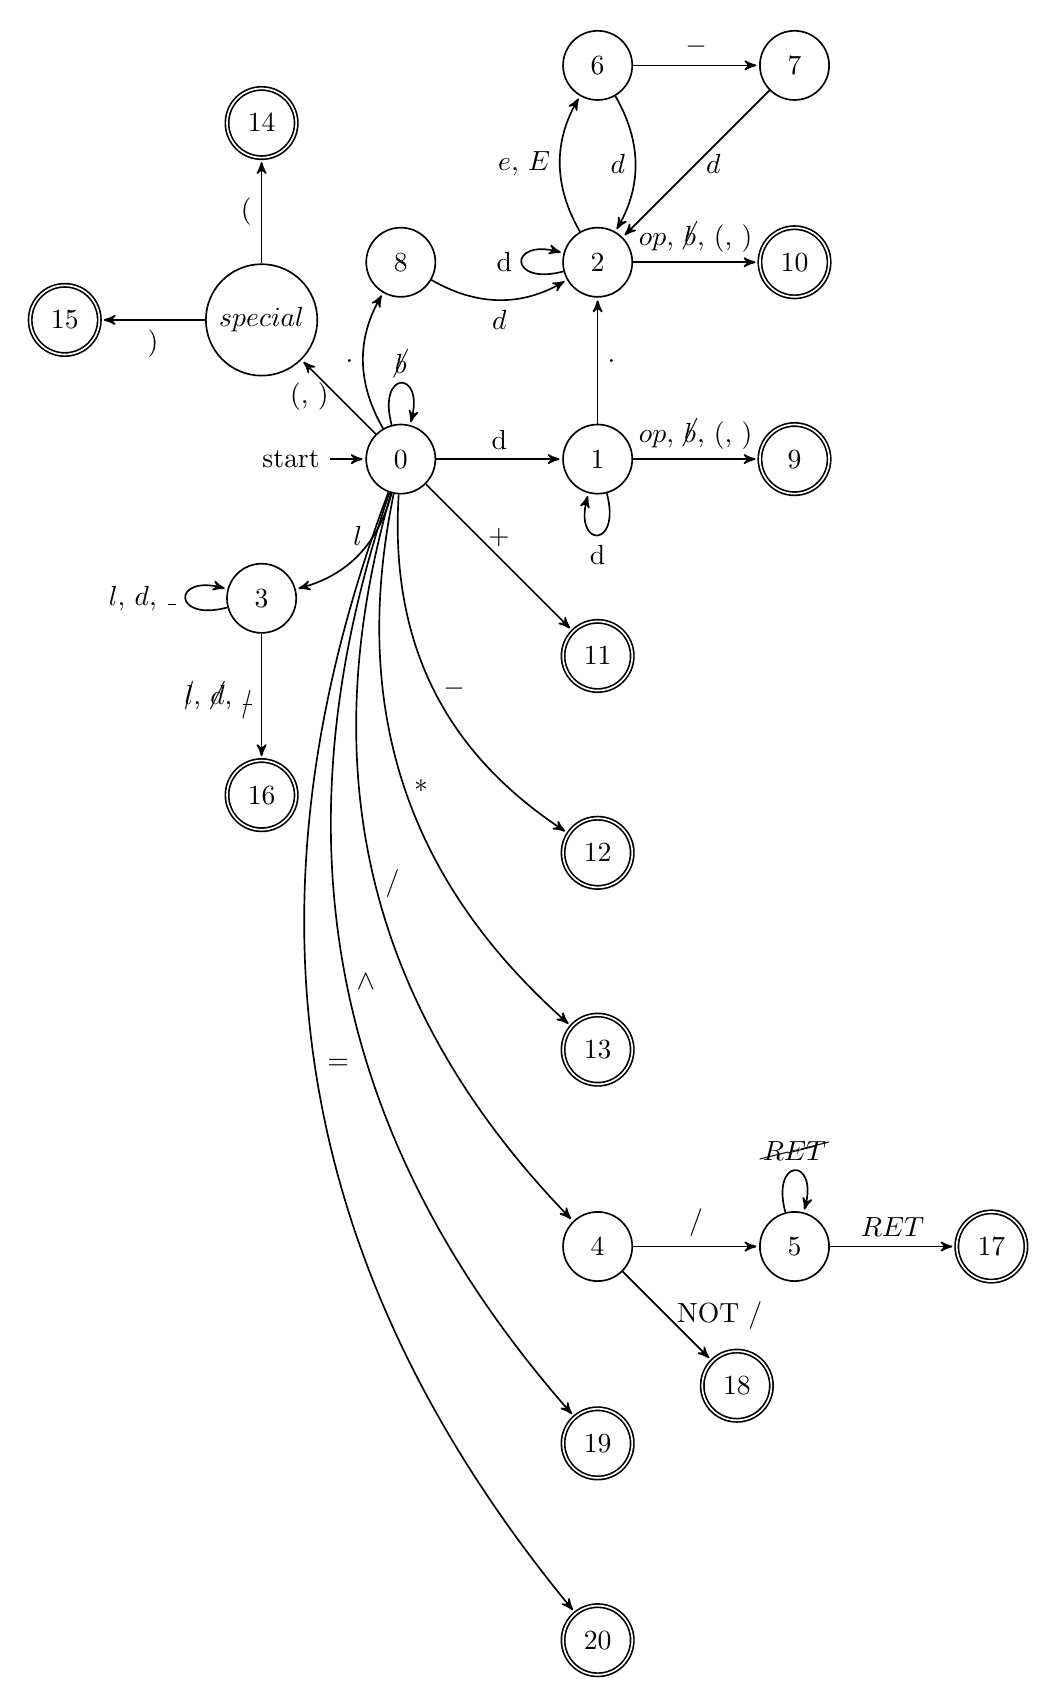
\begin{tikzpicture}[->, >=stealth', shorten >=1pt, auto, node distance=2.5cm, semithick]
    \node[state, initial] (0) {$0$};
    \node[state, right of=0] (1) {$1$};
    \node[state, accepting, right of=1] (int) {$9$};
    \node[state, above of=1] (3) {$2$};
    \node[state, accepting, right of=3] (real) {$10$};
    \node[state, accepting, below of=1] (add) {$11$};
    \node[state, accepting, below of=add] (sub) {$12$};
    \node[state, accepting, below of=sub] (mul) {$13$};
    \node[state, below of=mul] (6) {$4$};
    \node[state, accepting, below right of=6] (truediv) {$18$};
    \node[state, accepting, below of=6] (pow) {$19$};
    \node[state, accepting, below of=pow] (asign) {$20$};
    \node[state, above left of=0] (special) {$special$};
    \node[state, accepting, above of=special] (open) {$14$};
    \node[state, accepting, left of=special] (close) {$15$};
    \node[state, below left of=0] (5) {3};
    \node[state, accepting, below of=5] (var) {$16$};
    \node[state, right of=6] (7) {5};
    \node[state, accepting, right of=7] (com) {$17$};
    \node[state, above of=3] (8) {6};
    \node[state, right of=8] (9) {7};
    \node[state, above of=0] (10) {8};


    \draw (0) edge[loop above] node{$\cancel{b}$} (0)
          (0) edge[above] node{d} (1)
          (1) edge[loop below] node{d} (1)
          (1) edge[above] node{$op$, $\cancel{b}$, $($, $)$} (int)
          (1) edge[right] node{$.$} (3)
          (0) edge[bend left, left] node{$.$} (10)
          (10) edge[bend right, below] node{$d$} (3)
          (3) edge[loop left] node{d} ()
          (3) edge[above] node{$op$, $\cancel{b}$, $($, $)$} (real)
          (0) edge[above] node{$+$} (add)
          (0) edge[bend right, right] node{$-$} (sub)
          (0) edge[bend right, right] node{$*$} (mul)
          (0) edge[bend right, right] node{$/$} (6)
          (6) edge[right] node{NOT $/$} (truediv)
          (6) edge[above] node{$/$} (7)
          (7) edge[loop above] node{$\cancel{RET}$} (7)
          (7) edge[above] node{$RET$} (com)
          (0) edge[bend right, right] node{$\wedge$} (pow)
          (0) edge[bend left, above] node{$l$} (5)
          (5) edge[loop left] node{$l$, $d$, $\_$} (5)
          (5) edge[left] node{$\cancel{l}$, $\cancel{d}$, $\cancel{\_}$} (var)
          (0) edge[left] node{$($, $)$} (special)
          (special) edge[left] node{$($} (open)
          (special) edge[below] node{$)$} (close)
          (0) edge[bend right] node{$=$} (asign)
          (3) edge[bend left, left] node{$e$, $E$} (8)
          (8) edge[bend left, left] node{$d$} (3)
          (8) edge[above] node{$-$} (9)
          (9) edge[right] node{$d$} (3);



  \end{tikzpicture}
\end{center}

\end{document}
